\documentclass{standalone}
%\documentclass[convert={density=600,size=1080x800,outext=.png}]{standalone}
%\documentclass[convert={outext=.jpg}]{standalone}
\NeedsTeXFormat{LaTeX2e}
\usepackage{tikz}
\usepackage[utf8]{inputenc}
\usepackage{wasysym}
% \usepackage{fontspec}


\newcommand\Name            {Test/0001}  % Name
\newcommand\Crystal         {INTRI~5422} % Crystal number
\newcommand\HEAD            {1.59}       % HEAD conc x 10^10
\newcommand\TAIL            {1.60}       % TAIL conc x 10^10

\newcommand\Scale{4} % Scale
\newcommand\Dia{50} % Detector diameter in mm
\newcommand\Hei{20} % Detector hight in mm
\newcommand\Gdt{2} % Groove depth
\newcommand\Bult{1} %widow bulletization
\newcommand\FltD{10} %Flat Contact diam 
\newcommand\GrvEx{28} %Groove ext. diameter
\newcommand\GrvIn{15} %Groove int. diameter



\newcommand\Diam{\Dia/\Scale} % Detector diameter in mm
\newcommand\Height{\Hei/\Scale} % Detector hight in mm
\newcommand\WO{\Gdt/\Scale} % Groove depth
\newcommand\Bullet{\Bult/\Scale} %widow bulletization
\newcommand\FCD{\FltD/\Scale} %Flat Contact diam 
\newcommand\GrooveExt{\GrvEx/\Scale} %Groove ext. diameter
\newcommand\GrooveInt{\GrvIn/\Scale} %Groove int. diameter

\tikzset{
  arrow/.style={<->,>=latex,thin,gray,every rectangle node/.style={fill=white,midway,font=\sffamily}},
  dimen/.style={thin,gray},
  caption/.style={font=\sffamily,gray},
}
\begin{document}

    
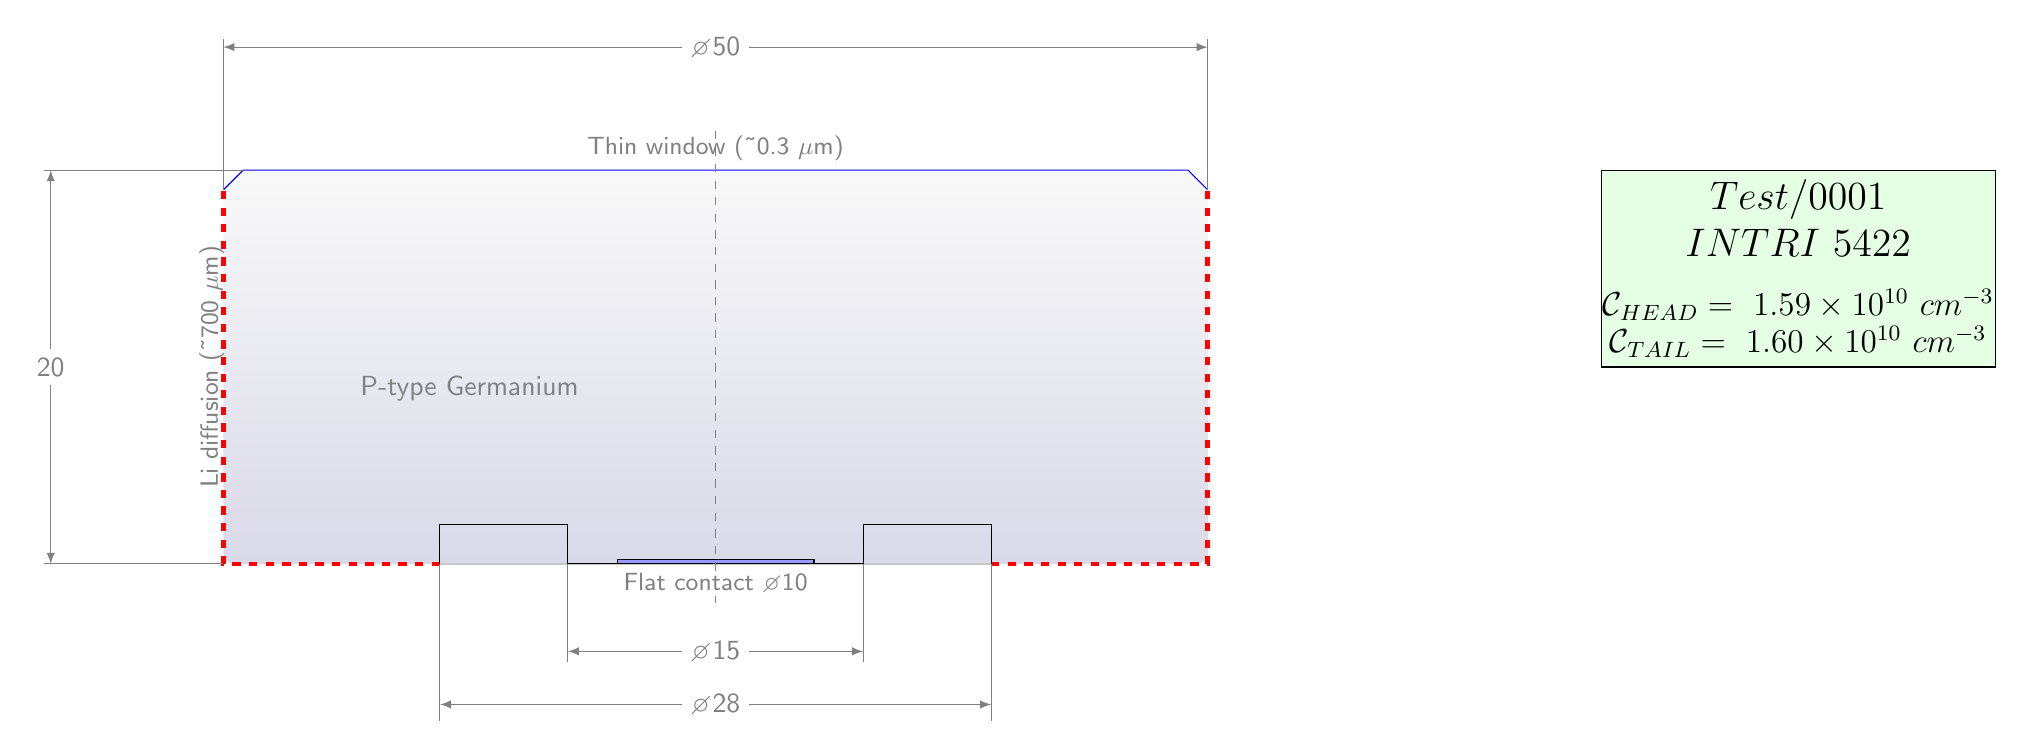
\begin{tikzpicture}
  % Back fill
  \draw[rounded corners, top color=gray!5!white, bottom color=black!60!blue!15,draw=none] (0,-\Height) -- (0,-\Bullet) --
  (\Bullet,0) -- (\Diam-\Bullet,0) -- (\Diam,-\Bullet) -- (\Diam,-\Height) -- cycle;
  \draw[gray!45, line width=0.5pt] (\Diam/2 - \FCD/2,-\Height) -- (\Diam/2 + \FCD /2,-\Height);
  \draw[gray!45, line width=0.5pt] (\Diam/2 +\GrooveExt/2,-\Height) -- (\Diam/2 + \FCD /2,-\Height);
  \draw[gray!45, line width=0.5pt] (\Diam/2 -\GrooveExt/2,-\Height) -- (\Diam/2 - \FCD /2,-\Height);
% ---
    \draw[red,ultra thick,dashed] (\Diam/2-\GrooveExt/2,-\Height) -- (0,-\Height) -- (0,-\Bullet); %Left wall
    \draw[red,ultra thick,dashed] (\Diam/2+\GrooveExt/2,-\Height) -- (\Diam,-\Height) -- (\Diam,-\Bullet); %Right wall
    \draw[blue,thin] (0,-\Bullet) -- (\Bullet,0) %bulletize left
     -- (\Diam-\Bullet,0) -- (\Diam,0-\Bullet); %bulletize right
    \draw[thin] (\Diam/2 +\GrooveExt/2,-\Height) -- (\Diam/2 +\GrooveExt/2,-\Height+\WO) -- 
      (\Diam/2 +\GrooveInt/2,-\Height+\WO) -- (\Diam/2 +\GrooveInt/2,-\Height) -- (\Diam/2 + \FCD /2,-\Height);  %Groove right
    \draw[thin] (\Diam/2 -\GrooveExt/2,-\Height) -- (\Diam/2 -\GrooveExt/2,-\Height+\WO) -- 
      (\Diam/2 -\GrooveInt/2,-\Height+\WO) -- (\Diam/2 -\GrooveInt/2,-\Height) -- (\Diam/2 - \FCD /2,-\Height);  %Groove left
    % \draw[blue,thick](\Diam/2 - \FCD /2,-\Height) -- (\Diam/2 + \FCD /2,-\Height); % Flat Contact
    \filldraw[fill=blue!40!white, draw=black] (\Diam/2 - \FCD /2,-\Height) rectangle (\Diam/2 + \FCD /2,-\Height + 0.2/\Scale);
    \draw[gray,thin,dashed,opacity=5] (\Diam/2,\Height/10) -- (\Diam/2,-\Height - \Height/10); %Symmetry line
    %--------Captions--------
    \draw (\Diam/2, -\Height)node[caption,anchor=north]{\small Flat contact $\diameter$\pgfmathparse{int(\FltD)}\pgfmathresult};
    \draw (\Diam/2, 0) node[caption,anchor=south]{\small Thin window (\char`\~ 0.3 $\mu$m)};
    \draw (-0.6/\Scale, -\Height*0.5) node[caption,anchor=center,rotate=90]{\small Li diffusion (\char`\~ 700 $\mu$m)};
    \draw (\Diam/4, -\Height/1.8) node[caption,anchor=center]{P-type Germanium};
    %--------Sizes--------
    \draw[dimen] (0,-\Bullet) -- (0,\Height/3);
    \draw[dimen] (\Diam,-\Bullet) -- (\Diam,\Height/3); %---diameter---
    \draw[arrow,<->] (0,\Height/3.2) -- (\Diam,\Height/3.2) node{$\diameter$\pgfmathparse{int(\Dia)}\pgfmathresult};
    %---
    \draw[dimen] (\Bullet,0) -- (-\Diam/5.5,0);
    \draw[dimen] (0,-\Height) -- (-\Diam/5.5,-\Height); %---height---
    \draw[arrow,<->] (-\Diam/5.7,0) -- (-\Diam/5.7,-\Height) node{\pgfmathparse{int(\Hei)}\pgfmathresult};
    %---
    \draw[dimen] (\Diam/2-\GrooveInt/2,-\Height) -- (\Diam/2-\GrooveInt/2,-\Height-\Height/4);
    \draw[dimen] (\Diam/2+\GrooveInt/2,-\Height) -- (\Diam/2+\GrooveInt/2,-\Height-\Height/4); %---Groove inner D---
    \draw[arrow,<->] (\Diam/2-\GrooveInt/2,-\Height -\Height/4.5) -- (\Diam/2+\GrooveInt/2,-\Height - \Height/4.5) node{$\diameter$\pgfmathparse{int(\GrvIn)}\pgfmathresult};
    %---
    \draw[dimen] (\Diam/2-\GrooveExt/2,-\Height) -- (\Diam/2-\GrooveExt/2,-\Height-\Height/2.5);
    \draw[dimen] (\Diam/2+\GrooveExt/2,-\Height) -- (\Diam/2+\GrooveExt/2,-\Height-\Height/2.5); %---Groove inner D---
    \draw[arrow,<->] (\Diam/2-\GrooveExt/2,-\Height -\Height/2.8) -- (\Diam/2+\GrooveExt/2,-\Height - \Height/2.8) node{$\diameter$\pgfmathparse{int(\GrvEx)}\pgfmathresult};
    %---
    %\draw[dimen] (\Diam-\Bullet,0) -- (\Diam*1.2,0);

    %--- INFO BOX
    \newcommand\LX{\Diam/2.5}           % Legend box horizontal size
    \newcommand\LY{\LX/2}               % Legend box vertical size
    \newcommand\Xa{\Diam*1.4}           % Legend box horizontal position
    \newcommand\Ya{0/\Scale}            % Legend box vertical position

    \filldraw[left color=green!10, right color=green!10, draw=black] (\Xa, \Ya) rectangle (\Xa+\LX, \Ya-\LY);
    \draw (\Xa+\LX/2, \Ya) node[anchor=north]{\Large $\Name$};
    \draw (\Xa+\LX/2, \Ya-\LY/4) node[anchor=north]{\Large $\Crystal$};
    \draw (\Xa+\LX/2, \Ya-\LY/1.8) node[anchor=north]{\large $\mathcal{C}_{HEAD}=~\HEAD\times10^{10}~cm^{-3}$};
    \draw (\Xa+\LX/2, \Ya-\LY) node[anchor=south]{\large $\mathcal{C}_{TAIL}=~\TAIL\times10^{10}~cm^{-3}$};
    %---

  \end{tikzpicture}

\end{document}
